\documentclass{beamer}
\usepackage[utf8]{inputenc}
\usepackage[russian]{babel}
\usepackage{caption}
\usepackage{listings}
\usepackage{relsize}
\usetheme{Antibes}
\usecolortheme{seahorse}
\setbeamercovered{transparent}
\captionsetup[figure]{labelformat=empty}
\captionsetup[figure]{justification=centering}
\lstset{keywordstyle=\color{blue}\bfseries}
\lstset{basicstyle=\scriptsize}

\title[Введение в функциональное программирование]{Обзор курса}
\author{Олег Смирнов\\
\texttt{oleg.smirnov@gmail.com}}
\institute{УНК ``ИПСА'' НТУУ ``КПИ''}
\date{\today}
\begin{document}

\begin{frame}
\titlepage
\end{frame}

\begin{frame}{Программа на сегодня}
  \begin{itemize}
    \item Вводная лекция и обзор курса
    \item Первая лекция -- итеративные и рекурсивные процессы
  \end{itemize}
\end{frame}

\begin{frame}{Немного об авторе}
  \begin{itemize}
  \item {\bf 1999-2005:} Факультет прикладной математики КПИ
  \item {\bf 2003-2005:} x86 Asm, C; reverse engineering, системное программирование
  \item {\bf 2005-2009:} C++, Perl, Python; распределённые системы, сетевые протоколы
  \item {\bf 2009-2010:} Системы поддержки операций; курс алгоритмов в Global Logic
  \item {\bf 2011-сейчас:} Erlang, Ocaml; высоконагруженные системы, социальные сервисы
  \end{itemize}
\end{frame}

\begin{frame}{``Функциональщина'' глазами обычного программиста}
  \lstinputlisting[language=Haskell]{lecture0/quine.hs}
\end{frame}

\begin{frame}{``Функциональщина'' глазами обычного программиста}
\begin{figure}
   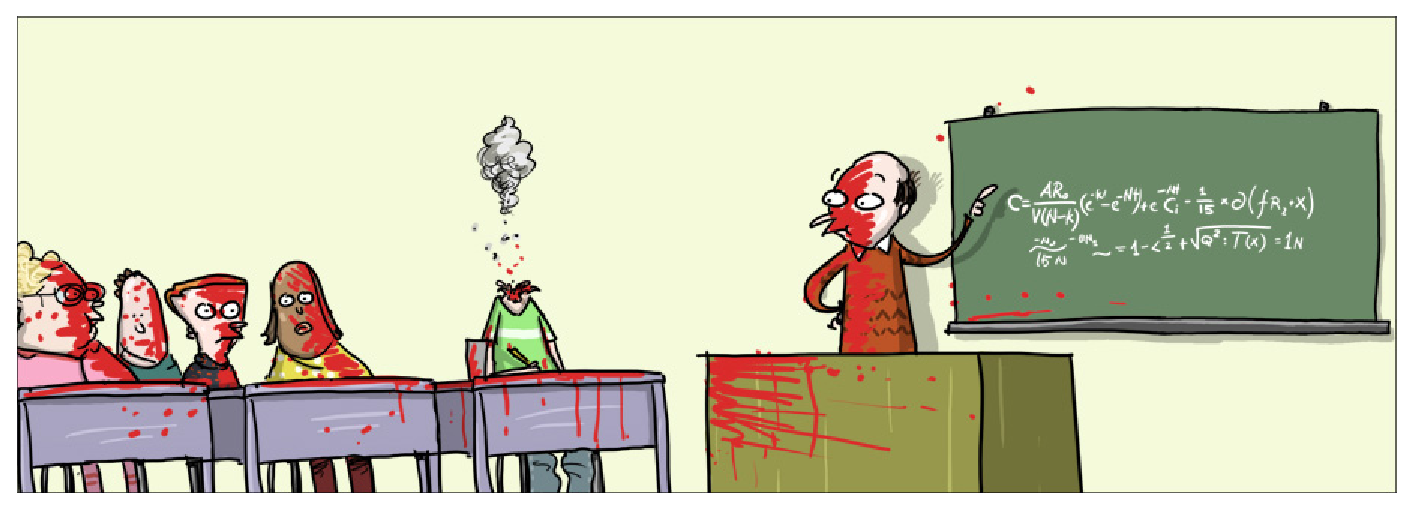
\includegraphics[scale=0.44]{lecture0/Matematik-Hjerne-Formel-WM_strip_DK_20090625.eps}
\end{figure}
\end{frame}

\begin{frame}{Цели курса}
  \begin{enumerate}
  \item Практика функционального программирования
  \uncover<0>{
  \item Изучение новой парадигмы
  \item Приёмы функционального программирования
  }
  \end{enumerate}
\end{frame}

\begin{frame}{Практика функционального программирования}
  \begin{figure}[h]
    \begin{minipage}[h]{0.49\linewidth}
      \begin{center}
        
\includegraphics[height=12mm]{lecture0/Barcap-logo.eps}
      \end{center}
    \end{minipage}
    \begin{minipage}[h]{0.49\linewidth}
      \begin{center}
        
\includegraphics[height=18mm]{lecture0/logo_grammarly.eps}
      \end{center}
    \end{minipage}
  \end{figure}
  \begin{figure}
    
\includegraphics[height=15mm]{lecture0/janestreet.eps}
  \end{figure}
  \begin{figure}[h]
    \begin{minipage}[h]{0.49\linewidth}
      \begin{center}
        
\includegraphics[height=13mm]{lecture0/Massive_Solutions.eps}
      \end{center}
    \end{minipage}
    \begin{minipage}[h]{0.49\linewidth}
      \begin{center}
        
\includegraphics[height=13mm]{lecture0/Socialabs.eps}
      \end{center}
    \end{minipage}
  \end{figure}
\end{frame}

\begin{frame}{Цели курса}
  \begin{enumerate}
  \item Практика функционального программирования
  \item Изучение новой парадигмы
  \uncover<0>{
  \item Приёмы функционального программирования
  }
  \end{enumerate}
\end{frame}

\begin{frame}[fragile]{Изучение новой парадигмы}  
  \begin{minipage}[t]{0.49\linewidth}
    \begin{center}
      \lstinputlisting[language=Java]{lecture0/fact.cs}      
    \end{center}
  \end{minipage}
  \begin{minipage}[t]{0.49\linewidth}
    \begin{center}
      \lstinputlisting[language=Caml]{lecture0/fact.fs}
    \end{center}
  \end{minipage}
\end{frame}

\begin{frame}{Изучение новой парадигмы}
  \begin{itemize}
  \item Неизменяемое состояние -- меньше ошибок, чище код\pause
  \item Верификация -- доказываем программы как теоремы\pause
  \item Параллелиризм -- технология Google MapReduce и Apache Hadoop
  \end{itemize}
\end{frame}

\begin{frame}{Параллелиризм}
  \begin{figure}[h]
    \begin{minipage}[h]{1\linewidth}
      \begin{center}
        
\includegraphics[height=10mm]{lecture0/GoogleLabs.eps}
        \caption{Jeffrey Dean and Sanjay Ghemawat. 2004. MapReduce: simplified data processing on large clusters. In \emph{Proceedings of the 6th conference on Symposium on Opearting Systems Design \& Implementation - Volume 6} (OSDI'04), Vol. 6. USENIX Association, Berkeley, CA, USA, 10-10.}
      \end{center}
    \end{minipage}
    \begin{minipage}[h]{1\linewidth}
      \begin{center}
        
\includegraphics[height=10mm]{lecture0/HadoopMR.eps}
        \caption{Mike Cafarella and Doug Cutting. 2004. Building Nutch: Open Source Search. \emph{Queue 2}, 2 (April 2004), 54-61.}        
      \end{center}
    \end{minipage}
  \end{figure}
\end{frame}

\begin{frame}{Цели курса}
  \begin{enumerate}
  \item Практика функционального программирования
  \item Изучение новой парадигмы
  \item Приёмы функционального программирования
  \end{enumerate}
\end{frame}

\begin{frame}{Приёмы функционального программирования}
  \begin{itemize}
  \item Сборка мусора: появилась в LISP (1958), стала мэйнстримом в 1995
    (Java)\pause
  \item Замыкания: появились в Scheme (1975), стали мэйнстримом в 2000-х
    (C\#, JavaScript)\pause
  \item Ленивая обработка: появилась в Miranda (1985), стала мэйнстримом
    в 2000-е (LINQ)
  \end{itemize}
\end{frame}

\begin{frame}{Приёмы функционального программирования}
  \begin{itemize}
  \item Параметрический полиморфизм: появился в 1983, сейчас мэйнстрим в
    Java, C\#, C++\pause
  \item Функции высшего порядка: появились в LISP, сейчас мэйнстрим везде,
    кроме Java\pause
  \item Вывод типов: появился в ML (1979), стал мэйнстримом в 2007
    (C\#, Scala, C++0x)
  \end{itemize}
\end{frame}

\begin{frame}{Программа курса: первый семестр}
  \begin{itemize}
    \item Язык F\#\pause
    \item Азы: рекурсия, функции высших порядков, замыкания, алгебраические
      типы данных\pause
    \item Практика: простые алгоритмы и структуры данных, парсинг\pause
    \item Параллельное программирование: свёртки, пробеги и технология MapReduce
  \end{itemize}
\end{frame}

\begin{frame}{Программа курса: второй семестр}
  \begin{itemize}
    \item Язык Haskell\pause
    \item Чисто функциональный структуры данных и персистентность\pause
    \item Программирование с монадами\pause
    \item Классы типов\pause
    \item Математические основы ФП и начало теории типов
  \end{itemize}
\end{frame}

\begin{frame}{Administrativia}
  \begin{itemize}
  \item Два семестра по шестнадцать лекций
  \item Восемь лабораторных, две контрольные и два экзамена\pause
  \item Лекции по пятницам на пятой паре (16:10) в аудитории 02-13\pause
  \item Два лектора плюс гостевые лекции\pause
  \item Программа курса: \url{http://goo.gl/RnbdH}
  \end{itemize}
\end{frame}

\begin{frame}{Учебники}
  \begin{figure}[h]
    \begin{minipage}[h]{0.49\linewidth}
      \begin{center}
          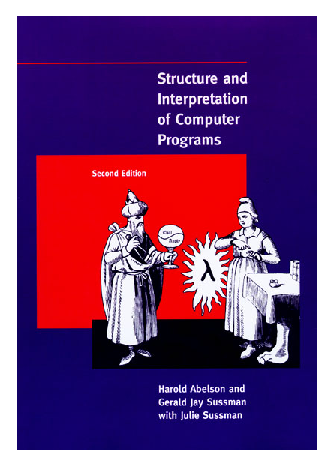
\includegraphics[width=20mm]{lecture0/SICP.eps}
          \caption{Харольд Абельсон, Джеральд Джей Сассман
            ``Структура и интерпретация компьютерных программ''}
      \end{center}
    \end{minipage}
  \end{figure}
\end{frame}

\begin{frame}{Учебники}
  \begin{figure}[h]
    \begin{minipage}[h]{0.49\linewidth}
      \begin{center}
          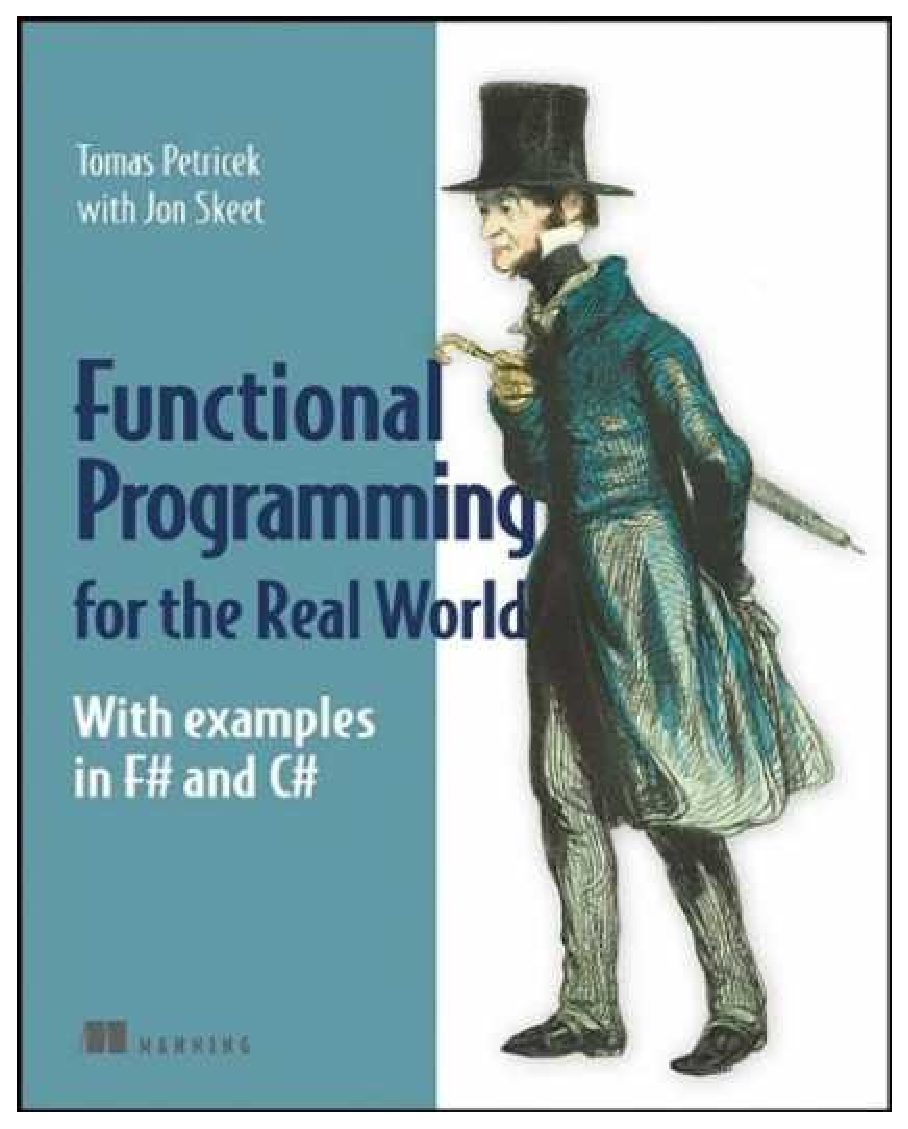
\includegraphics[width=20mm]{lecture0/FPiRW.eps}
          \caption{Томас Петричек, Джон Скит
            ``Functional Programming for the Real World''}
      \end{center}
    \end{minipage}
    \begin{minipage}[h]{0.49\linewidth}
      \begin{center}
        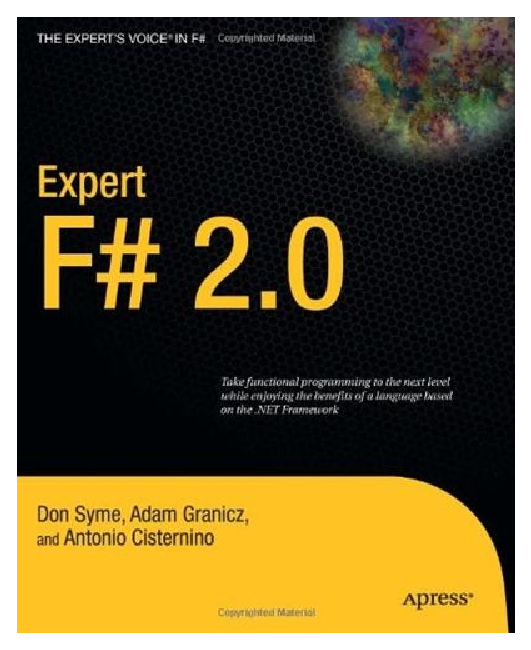
\includegraphics[width=20mm]{lecture0/Expert_Fsharp.eps}
        \caption{Дон Сайм ``Expert F\# 2.0''}
      \end{center}
    \end{minipage}
  \end{figure}
\end{frame}

\begin{frame}{Рекомендуемая литература}
  \begin{figure}
    \begin{minipage}{0.3\linewidth}
      \begin{center}
        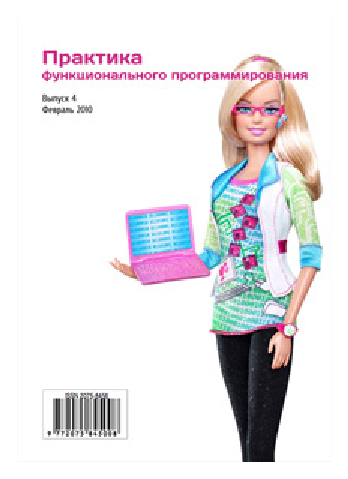
\includegraphics[width=20mm]{lecture0/pfp2010-04.eps}
      \end{center}
    \end{minipage}
    \begin{minipage}{0.3\linewidth}
      \begin{center}
        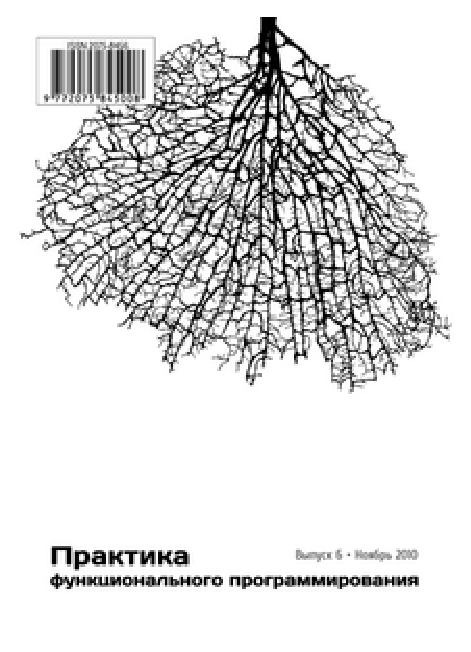
\includegraphics[width=20mm]{lecture0/pfp2010-06.eps}
      \end{center}
    \end{minipage}
    \begin{minipage}{0.3\linewidth}
      \begin{center}
        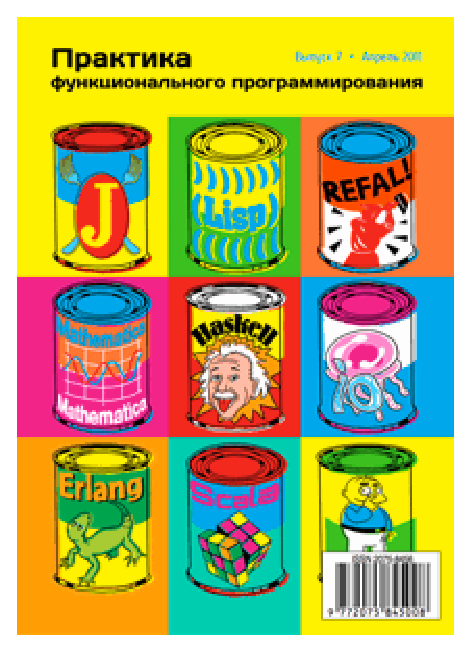
\includegraphics[width=20mm]{lecture0/pfp2011-07.eps}
      \end{center}
    \end{minipage}
    \caption{Журнал ``Практика функционального программирования''
      \url{http://fprog.ru}}
  \end{figure}
\end{frame}

\begin{frame}
  \begin{center}
    \LARGE{Вопросы?}
  \end{center}
\end{frame}

\end{document}

